\chapter{Planteamiento de la Solución}
\label{cap:planteamiento}
\section{Planteamiento inicial}

Una vez vistas las diferencias esenciales entre el sistema original que hemos heredado y las ampliaciones que hemos realizado durante el desarrollo del presente trabajo, se tratará las ideas iniciales de cómo pensábamos realizar el trabajo, indicando desde el punto de vista técnico, organizativo y general, la manera de afrontar este proyecto.

En cuanto a la organización, la planificación inicial era clara: invertir la mayor parte de los primeros meses investigando el proyecto, y a partir del final del primer cuatrimestre y durante todo el segundo cuatrimestre, realizar el trabajo de desarrollo completo del proyecto.

Esta primera fase de investigación fue larga y tediosa, ya que el tema de este TFG fue propuesto por los alumnos, sin una idea clara sobre qué objetivos podría tener el presente trabajo, pero sabiendo que el tema de las simulaciones multi agente es un campo muy interesante en el que profundizar. Durante estos primeros meses se realizaron lluvias de ideas y propuestas para los objetivos. Algunos de los primeros objetivos consistían en añadir funcionalidades a la aplicación o permitir a los usuarios modificarla más, pero decidimos pivotar para poder hacer la aplicación ya existente, más fácil de usar para perfiles no técnicos, así como centrarnos en extender ciertas funcionalidades para que sean más útiles para este tipo de perfiles, en lugar para programadores.

Entre las complejidades que se encontraron durante esta primera fase de investigación, se destacan las inconsistencias entre versiones de ciertas tecnologías, la comprensión de todo el código existente, o el aprendizaje de las tecnologías usadas en el desarrollo del proyecto, entre otras muchas. Además, al investigar sobre el tema, esta fue la fase en la que se desarrolló el capítulo del Estado de la Cuestión, lo que ayudó a tomar otra perspectiva acerca del proyecto.

Durante la segunda fase, una vez definidos y validados los primeros objetivos, e comenzó con todo el desarrollo del sistema. Caba destacar que en esta sección, muchas reconsideraciones tuvieron que ser realizadas, además de multitud de cambios en el código original como adaptaciones para que funcionen los nuevos cambios. Todo esto está explicado en las siguientes secciones.

En el transcurso de ambas fases, tuvimos reuniones regularmente con nuestros tutores, supervisando el estado del sistema, así como los avances, problemas y consideraciones que tuviéramos que tener en cuenta. En un principio estas reuniones eran más espaciadas en el tiempo, haciendo una o dos al mes, y en la fase de desarrollo, donde avanzábamos más rápido, las reuniones eran semanales o cada dos semanas para estar al día del proyecto.



\subsection{Estado tecnológico inicial del sistema}

En esta sección se analizará, a grandes rasgos, el estado inicial desde el punto de vista técnico del proyecto. Es decir, el diseño y situación que había inicialmente para ejecutar el sistema, para que en las próximas secciones se entiendan los cambios realizados y el porqué de estos.

En cuanto al diseño, originalmente, existían 2 backends. El primero de ellos era el backend de Django, el cual era el encargado de gestionar todas las llamadas del frontend, o interfaz, que inicialmente no eran muchas, ya que el frontend solamente servía como apoyo para poder visualizar las simulaciones. 

El segundo backend era el de reverie, como lo llaman los autores del código. Este se encargaba de procesar todos los comandos que los usuarios deseaban ejecutar, calculaba el resultado de estos y se comunicaba con el backend de django para que procesase el resultado de las ejecuciones y se reflejara en la interfaz.

\begin{figure}[h]
	\centering
	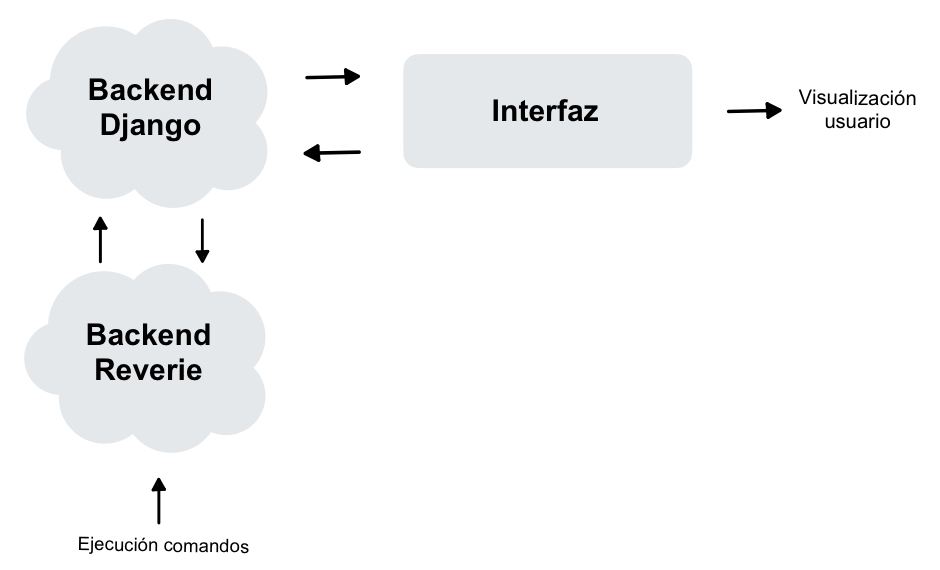
\includegraphics[width = 0.9\textwidth]{Imagenes/Vectorial/disenoSistemaOriginal.jpeg}
	\caption{Diseño del sistema original}
	\label{fig:sistemaOriginal}
\end{figure}

Como se puede ver en la figura \ref{fig:sistemaOriginal}, se ve reflejado el estado del sistema desde el punto del diseño. El flujo habitual sería el siguiente:

\begin{enumerate}
	\item El usuario iría a la terminal en la que se está ejecutando el backend de reverie (que gestiona todas las llamadas a los modelos de lenguaje) y ejecutaría alguno de los comandos (run, whisper, exit, save...)
	
	\item El backend de reverie realizaría la serie de llamadas al modelo de lenguaje pertinentes, así como la organización de las respuestas y almacenamiento de las mismas, y pasaría el resultado de la ejecución al backend de django
	
	\item El backend de Django, con la nueva información obtenida de reverie, adaptaría la información a un formato para que pueda ser procesado en el frontend
	
	\item Se procesaría la información de django en el frontend y se enseñaría al usuario final. Como se ha mencionado, el usuario no podría interactuar con esta información para realizar llamadas al backend desde la interfaz, sino que tendría que acudir a la terminal de reverie para comunicarse
	
\end{enumerate}

También es importante resaltar que para realizar acciones como crear una simulación, ver una simulación existente o interactuar con ella, todas las acciones debían ser realizadas mediante la terminal. La interfaz estaba relegada únicamente a mostrar el resultado de la simulación.

\section{Ajustes y reconsideraciones}

En esta sección se tratarán las adaptaciones que se han ido adoptando durante el desarrollo del proyecto, indicando así cómo han ido cambiando distintas facetas del sistema, tanto en su planificación como en su implementación técnica.

Este análisis permitirá comprender mejor la evolución del proyecto, los desafíos enfrentados y las soluciones implementadas. Además, revelará la capacidad de adaptación y el aprendizaje continuo que han sido fundamentales para el éxito del proyecto.

\subsection{Cambios en los objetivos}

Inicialmente, se fijaron una serie de objetivos sin tener un conocimiento claro sobre la arquiterctura y funcionamiento del sistema. Estos objetivos estaban enfocados en la extensibilidad y modificación de lo previamente existente. A grandes rasgos, los objetivos inicialmente marcados eran los siguientes:

\begin{enumerate}
	\item Añadir uno o varios mapas complementarios a mayores del existente, además de poder modificar las apariencias, nombres y personalidades de los agentes de la simulación
	
	\item Permitir la interacción directa con los agentes y el entorno, pudiendo clicar directamente sobre el mapa y que se reconociese el objeto que se estaba indicando, para así poder modificar su estado (indicar que se está quemando el objeto, por ejemplo)
	
	\item Permitir a los usuarios utilizar su propio modelo del lenguaje, ya sea descargado en local o empleando diferentes APIs externas alternativas al modelo del lenguaje original
\end{enumerate}

Tras evaluar todo el sistema, se decidió pivotar sobre estos objetivos iniciales, ya que conllevaban una gran cantidad de trabajo y apenas aportaban valor añadido al programa original, por lo que se propusieron unos nuevos objetivos, sobre los cuales se ha construído la base de los objetivos finales que se pueden consultar en la introducción de este documento. El resultado de pivotar los objetivos fue, en líneas generales, el siguiente:

\begin{enumerate}
	\item Modificación de las personalidades de los personajes, enfocándose así en la importancia de crear nuevas simulaciones con distintas relaciones sociales, siendo agnósticos al mapa e imagen de los agentes, ya que cambiar esto no aporta tanto valor
	
	\item Interacción en tiempo real con los agentes, mediante un menú en el que poder entrevistar al personaje, así como crearle inquietudes y nuevas memorias para ver cómo reacciona
	
	\item Generación automática de resúmenes
	
	\item Englobar todas las funcionalidades en una interfaz sencilla e intuitiva
\end{enumerate}

\subsection{Limpieza de archivos del repositorio}
\label{limpiezaArchivos}

Al haber heredado el sistema original, realizado por terceros, pudimos apreciar que este, además de no ser extensible, tenía multitud de carpetas, archivos y funciones que no estaban siendo utilizados a día de hoy para nada en el proyecto, o que habían sido utilizados únicamente para depurar el código y lo habían olvidado. Por ello, decidimos limpiar todos estos datos innecesarios y dejar el sistema más limpio y sencillo, para que sea más sencilla la extensibilidad del mismo en el futuro.

En esta sección hemos recogido algunas de estas piezas de código que hemos eliminado, explicando qué hacían y el porqué de su eliminación:

\begin{itemize}
	\item \textbf{Carpeta \textit{path\_tester}:} Contenía un archivo como el main\_script.html y una vista especial que los desarrolladores usaron para depurar el código de las colisiones de los personajes con los bordes del mapa. No tenía utilidad ahora, solo a la hora de depurar esto en su momento
	
	\item \textbf{Función \textit{replay} del archivo \textit{views.py}:} Era una función que gestionaba la visualización de repeticiones de simulaciones. Estas eran similares a la demo de las simulaciones, pero con propósito de depuración de la vista de ejecución de simulación, por lo que no tenía ya valor
	
	\item \textbf{Carpeta \textit{persona\_state} y funciones asociadas:} En esta carpeta estaban los datos para poder ver en tiempo real todos los parámetros que afectaban a cada uno de los personajes. Esta información solo era usado en las repeticiones, que eliminamos del sistema
	
	\item \textbf{Entornos virtuales preexistentes:} Los desarrolladores de la aplicación inicial, dejaron sus propios entornos virtuales que habían usado para la creación de este proyecto. Como es recomendable que cada persona instale su entorno virtual particular, decidimos eliminar estas carpetas ya que no estaban siendo utilizadas para nada
	
	\item \textbf{Ficheros \textit{admin.py, models.py y tests.py} de la carpeta translator:} Ya que estos eran archivos vacíos que no estaban siendo utilizados,  necesarios para la configuración inicial pero obsoletos en este punto
	
\end{itemize}

\subsection{Selección del modelo de lenguaje}

\textcolor{red}{A RELLENAR POR KEVIN HABLANDO DE PROBLEMAS CON LLMs}


\section{Problemas encontrados}

En esta sección se tratarán algunos de los problemas surgidos durante el desarrollo de todo el proyecto. Teniendo en cuenta el planteamiento inicial, y debido a que el tema tratado en este trabajo es una investigación novedosa implementada por terceros, surgieron varios problemas e imprevistos que tuvimos que superar y resolver.

\subsection{Llamadas al back end durante la simulación}

Uno de los principales problemas con el que nos encontramos fueron las dificultades de hacer llamadas al back end mientras se ejecutaba una simulación. Esto era debido a que, mientras una simulación se ejecuta, en la interfaz se puede ver el mapa con todos los personajes, ejecutando las acciones en cada momento. Este mapa se renderiza y ejecuta utilizando la tecnología de Phaser, un framework usado para desarrollar videojuegos usando HTML.

Al usar este framework, como utiliza los botones del teclado para interactuar con el mapa (como las flechas para mover la cámara por el mapa, por ejemplo), uno de los botones que están "reservados" por Phaser es el de la barra espaciadora, lo que hacía que no se pudiesen enviar susurros, ya que no permitía el sistema que se insertaran espacios.

Tras investigar y dar con la raíz del problema, se abrían varias opciones para solucionarlo. La primera era crear una nueva página solamente para los susurros, donde no interactuase con el motor de Phaser y así poder enviar los mensajes. Esta solución era simple y fácil de implementar, pero llegamos a la conclusión de que no tendría demasiado sentido, ya que crear una nueva vista únicamente para enviar un mensaje (sin esperar una respuesta por parte del personaje) no era ideal, ya que la experiencia de usuario cobra más sentido cuando puedes enviar el susurro mediante la interfaz de la simulación, abriendo un modal.

La segunda opción, y la que decidimos implementar finalmente, fue la de intentar pausar la ejecución de la simulación para que así Phaser "libere" los recursos y permita a los usuarios usar la barra espaciadora. Esto nos resultó con mayor sentido ya que así el usuario no tendría que estar constantemente cambiand entre vistas y resultaría en una mejor experiencia. Por tanto, implementamos unos botones para pausar y reanudar la simulación, que cuando se pulsan activan y desactivan otros ciertos botones. Por ejemplo, cuando se reanuda la simulación, no se permite al usuario chatear o susurrar con los personajes (se desactivan estos botones), pero cuando se pausa la simulación, el botón que se desactiva es el de ejecutar steps de la simulación.

\subsection{Acoplo de los personajes al mapa original}
\label{problemaPersonajes}
Como se ha mencionado en varias ocasiones, el sistema original no estaba pensado para ser extensible en multitud de aspectos. Uno de los aspectos más importantes es que todos los personajes tenían nombres, apariencias y personalidades predefinidas, lo que no permitía a los usuarios modificar los personajes y sus personalidades, por tanto, se verían encorsetados a siempre utilizar los mismos personajes con las mismas relaciones entre ellos y generar experimentos a partir de esto, lo cual limita muchísimo el uso de esta aplicación.

Uno de los mayores retos que nos propusimos fue despegar a los personajes de sus personalidades inherentes, para así poder hacer que los usuarios elijan las personalidades de cada uno y ver así los fenómenos sociales que aparecían.

Al no estar inicialmente pensado el sistema para esto, todos los nombres de los personajes, sus pensamientos, experiencias y objetos en el mapa, estaban directamente "hardcodeados" en el programa. Es decir, que estaban escritos directamente y no se permitía que se cambiasen.

El mayor problema fue hacer que los personajes fuesen agnósticos del mapa en el que se encontraban. El mapa inicial trataba de simular una villa, por lo que cada casa y cada objeto tenía el nombre de la familia o personaje que fuese su dueño, lo cual hacía muy fácil la interacción con los objetos de los distintos personajes. Nuestra solución fue que los personajes mantuviesen los nombres originales, pero que eso no influyese en la simulación, ya que ahora no importarían los objetos dentro de la simulación y los usuarios podrían decidir el contexto en el que se encuentran los persoajes, por lo que el mapa servirá ahora simplemente como un contenedor para visualizar la simulación.

\section{Conclusión final}

Tras ver el estado inicial en el que se encontraba el sistema, tanto desde un punto de vista técnico como desde un punto de vista más general, y teniendo en cuenta todos los problemas encontrados, realizando las reconsideraciones y ajustes necesarios, se termina con un sistema más robusto, usable y amigable.

Por tanto, en la figura \ref{fig:sistemaFinal}, se aprecia, a grandes rasgos, cómo ha cambiado el sistema desde el punto de vista del diseño a alto nivel, llevando a cabo los cambios previamente mencionados en las secciones pasadas.

\begin{figure}[h]
	\centering
	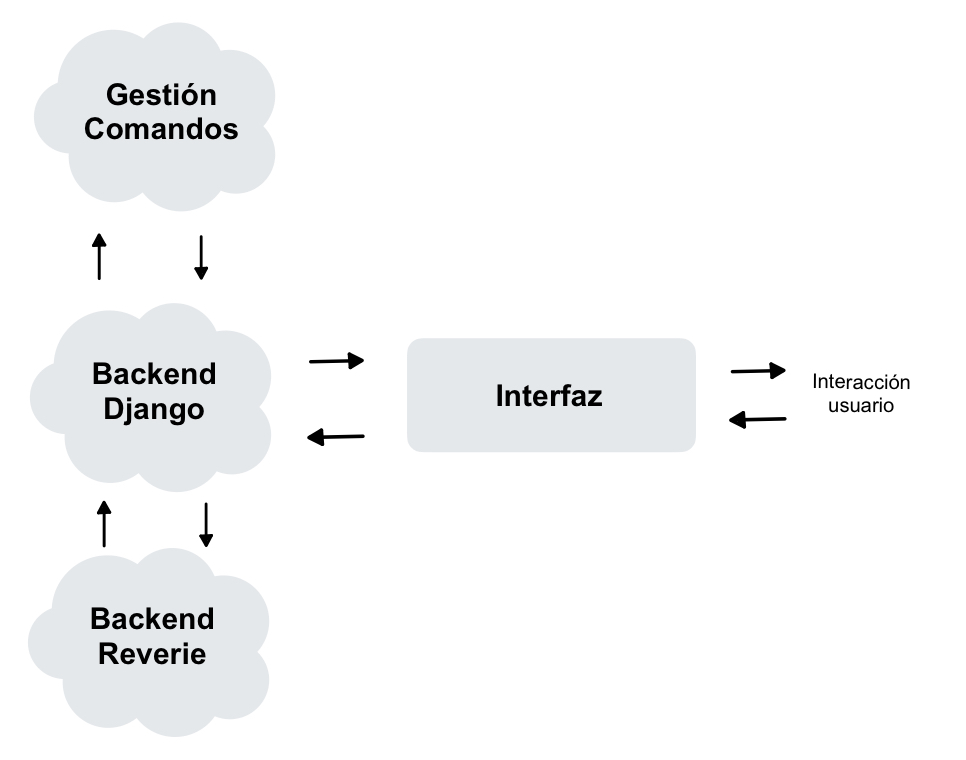
\includegraphics[width = 0.9\textwidth]{Imagenes/Vectorial/disenoSistemaFinal.jpeg}
	\caption{Diseño del sistema final tras las adaptaciones}
	\label{fig:sistemaFinal}
\end{figure}

Ahora, como se puede ver, hay un punto único de interacción entre el usuario y el sistema, que es mediante la interfaz. Así, interactuando con la interfaz los usuarios son capaces ahora de hacer lo mismo que antes y más, con las extensiones implementadas.

Mediante esta interacción, los usuarios pueden ejecutar todos los comandos, ver las simulaciones, crearlas e interactuar con ellas libremente.

El flujo de ejecución ahora es algo diferente:

\begin{enumerate}
	\item El usuario interactúa mediante la interfaz decidiendo la acción que desee
	
	\item Si el usuario desea ejecutar un comando de la simulación, se captará mediante la interfaz, se redirigirá al backend de django, el cual gestionará la llamada al gestor de comandos (nos permite ejecutar comandos mientras la aplicación sigue funcionando) y esta se encargará de llamar al backend de reverie para que ejecute el comando
	
	\item El backend de reverie devolverá la ejecución del comando a Django
	
	\item Al igual que antes, Django procesará esta información y la devolverá a la interfaz, donde el usuario podrá visualizarla y volver a interactuar con esta nueva información
	
\end{enumerate}
